\subsection{Construction de l'ensemble stable maximal : 2\up{ème} méthode}
Un autre algorithme pour le MIS a été proposée par les auteurs. C'est un algorithme distribué qui se résume en les étapes suivantes.
\begin{itemize}
\item Construire un arbre couvrant quelconque du graphe. (par le biais de messages)
\item Choisir une racine et stocker la distance à la racine (le rang) dans chaque point (par le biais de messages)
\item Colorer la racine en noir et envoyer un message noir a tout ses voisins dans le graphe (broadcast)
\item Lorsqu'un point reçoit un message noir, il change sa couleur en gris. Et envoie un message gris contenant son rang à tout ses voisins dans le graphe (broadcast)
\item Lorsqu'un point reçoit un message gris, il vérifie si le message gris viens d'un point au dessus de lui (de rang inférieur) dans l'arbre, dans ce cas il décrémente un compteur k (initialisé a son nombre de voisins dans le graphe de rang inférieur dans l'arbre). Lorsque ce compteur arrive à zéro il deviens noir et broadcast un message noir.
\item Des envois de messages supplémentaires permettent à l'algorithme distribué de notifier la racine de la fin de la procédure. Ils ne nous intéresseront pas.
\end{itemize}

\begin{figure}
\begin{center}
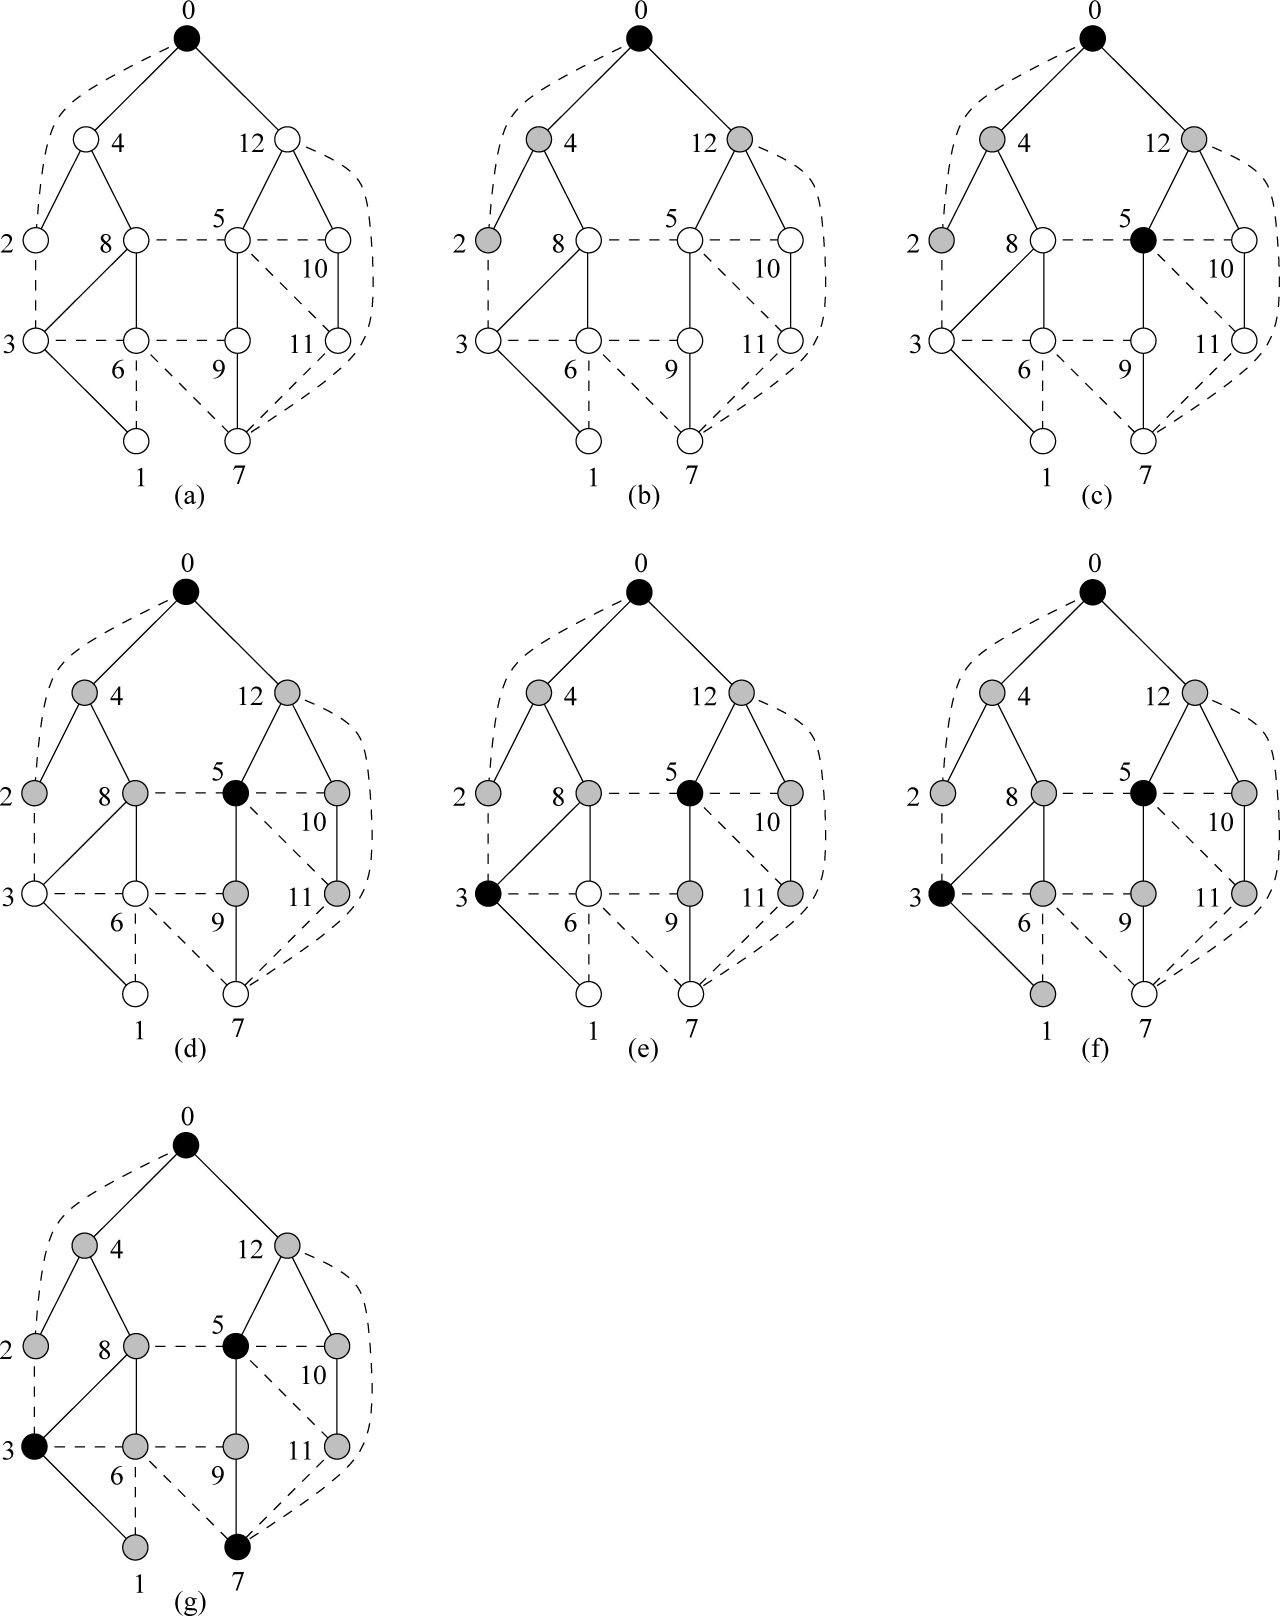
\includegraphics[scale=0.6]{images/figureMIS.jpg}
\caption{Construction du MIS}
\end{center}
\end{figure}

\paragraph{}
Notre implémentation consiste a traduire cet algorithme distribué en un algorithme classique :
\begin{itemize}
\item Pour l'arbre couvrant une implémentation inspirée de kruskal sans prendre en compte la longueur des segments et en utilisant des disjoint set
\item Une racine arbitraire est choisie et un parcours en profondeur de l'arbre est réalisé pour initialiser les rangs
\item Ensuite un parcours en largeur de l'arbre reproduira le mieux le comportement de l'algorithme distribué :
	\begin{itemize}
	\item On ajoute la racine dans une file puis tant que la file est non vide :
	\item On dépile la liste et on parcours les voisins du noeud dépilé
	\item On cherche un voisin noir : dans ce cas on change la couleur du noeud actuel en gris et on ajoute ses fils dans l'arbre dans la file
	\item Sinon on compte les voisins gris qui ont un rang inférieur au noeud actuel, on change sa couleur en noir et on ajoute ses fils dans l'abre dans la file 
	\end{itemize}
\item On retourne la liste des noeuds noirs
\end{itemize}

\paragraph{}
Il s'agit maintenant de donner une borne a la complexité de cet implémentation.

\paragraph{}
La construction de l'arbre couvrant consiste a parcourir tout les points du graphe. Pour chaque voisins n'étant pas dans le même Disjoint-Set (opération FIND), faire l'union de leur disjoint set avec celui du point considéré et construire la structure d'arbre (stocker les voisins du point dans l'arbre).
La complexité amortie des Disjoint Set optimisés peut être considérée comme constante. On réalise pour chaque point du graphe de degré d, au maximum d find et d union.

Soit $\Delta$ le degré maximal de notre graphe et $n$ le nombre de points. On est donc en $O(n \times \Delta)$.

L’initialisation des rang est un parcours en profondeur de l'arbre et dépends de l'étape précédente.
Le parcours en largeur effectué lors du reste de l'algorithme dépends aussi de la taille de l'arbre, chaque nœud à au maximum $\Delta -1$ fils et il y a $n$ nœuds

La complexité de cet algorithme est donc $O(n \times \Delta)$.
